\documentclass[]{article}
\usepackage{lmodern}
\usepackage{amssymb,amsmath}
\usepackage{ifxetex,ifluatex}
\usepackage{fixltx2e} % provides \textsubscript
\ifnum 0\ifxetex 1\fi\ifluatex 1\fi=0 % if pdftex
  \usepackage[T1]{fontenc}
  \usepackage[utf8]{inputenc}
\else % if luatex or xelatex
  \ifxetex
    \usepackage{mathspec}
  \else
    \usepackage{fontspec}
  \fi
  \defaultfontfeatures{Ligatures=TeX,Scale=MatchLowercase}
\fi
% use upquote if available, for straight quotes in verbatim environments
\IfFileExists{upquote.sty}{\usepackage{upquote}}{}
% use microtype if available
\IfFileExists{microtype.sty}{%
\usepackage{microtype}
\UseMicrotypeSet[protrusion]{basicmath} % disable protrusion for tt fonts
}{}
\usepackage[margin=1in]{geometry}
\usepackage{hyperref}
\hypersetup{unicode=true,
            pdftitle={Simulation of resampling method on chi-square distribution},
            pdfauthor={Xuelong Wang},
            pdfborder={0 0 0},
            breaklinks=true}
\urlstyle{same}  % don't use monospace font for urls
\usepackage{graphicx,grffile}
\makeatletter
\def\maxwidth{\ifdim\Gin@nat@width>\linewidth\linewidth\else\Gin@nat@width\fi}
\def\maxheight{\ifdim\Gin@nat@height>\textheight\textheight\else\Gin@nat@height\fi}
\makeatother
% Scale images if necessary, so that they will not overflow the page
% margins by default, and it is still possible to overwrite the defaults
% using explicit options in \includegraphics[width, height, ...]{}
\setkeys{Gin}{width=\maxwidth,height=\maxheight,keepaspectratio}
\IfFileExists{parskip.sty}{%
\usepackage{parskip}
}{% else
\setlength{\parindent}{0pt}
\setlength{\parskip}{6pt plus 2pt minus 1pt}
}
\setlength{\emergencystretch}{3em}  % prevent overfull lines
\providecommand{\tightlist}{%
  \setlength{\itemsep}{0pt}\setlength{\parskip}{0pt}}
\setcounter{secnumdepth}{5}
% Redefines (sub)paragraphs to behave more like sections
\ifx\paragraph\undefined\else
\let\oldparagraph\paragraph
\renewcommand{\paragraph}[1]{\oldparagraph{#1}\mbox{}}
\fi
\ifx\subparagraph\undefined\else
\let\oldsubparagraph\subparagraph
\renewcommand{\subparagraph}[1]{\oldsubparagraph{#1}\mbox{}}
\fi

%%% Use protect on footnotes to avoid problems with footnotes in titles
\let\rmarkdownfootnote\footnote%
\def\footnote{\protect\rmarkdownfootnote}

%%% Change title format to be more compact
\usepackage{titling}

% Create subtitle command for use in maketitle
\newcommand{\subtitle}[1]{
  \posttitle{
    \begin{center}\large#1\end{center}
    }
}

\setlength{\droptitle}{-2em}

  \title{Simulation of resampling method on chi-square distribution}
    \pretitle{\vspace{\droptitle}\centering\huge}
  \posttitle{\par}
    \author{Xuelong Wang}
    \preauthor{\centering\large\emph}
  \postauthor{\par}
      \predate{\centering\large\emph}
  \postdate{\par}
    \date{2018-10-23}

\usepackage{float,amsmath, bbm, siunitx, bm}
\floatplacement{figure}{H}
\newcommand{\indep}{\rotatebox[origin=c]{90}{$\models$}}

\begin{document}
\maketitle

{
\setcounter{tocdepth}{2}
\tableofcontents
}
\section{Motivation}\label{motivation}

The total estimation results of the Chi-square simulation is promising,
but when we applied the same method on the PCB data it did not show the
advantage as the Chi-square. One possible reason is the limits of the
sample size.

For the Chi-square simulation, we are able to generate the covariates
for each iteration. However, it is not true for the PCB data. The
alternative method of the random sample is to do the re-sampling on the
PCB data. But when the subet proportion is too small, the performance is
not that good. So it is the re-sampling procedure affect the proposed
method's result. Thus, we want to conduct a similar re-sampling
simulation as PCB data on simulated Chi-square data to see if there is a
significant difference on the method's result.

\section{Simulation setup}\label{simulation-setup}

All the steps are same as before, except this time we only sample the
chi-square data once, and then using subset of it to fit the model.

\subsection{p = 34}\label{p-34}

\subsubsection{fixed main and fixed interactive
effect}\label{fixed-main-and-fixed-interactive-effect}

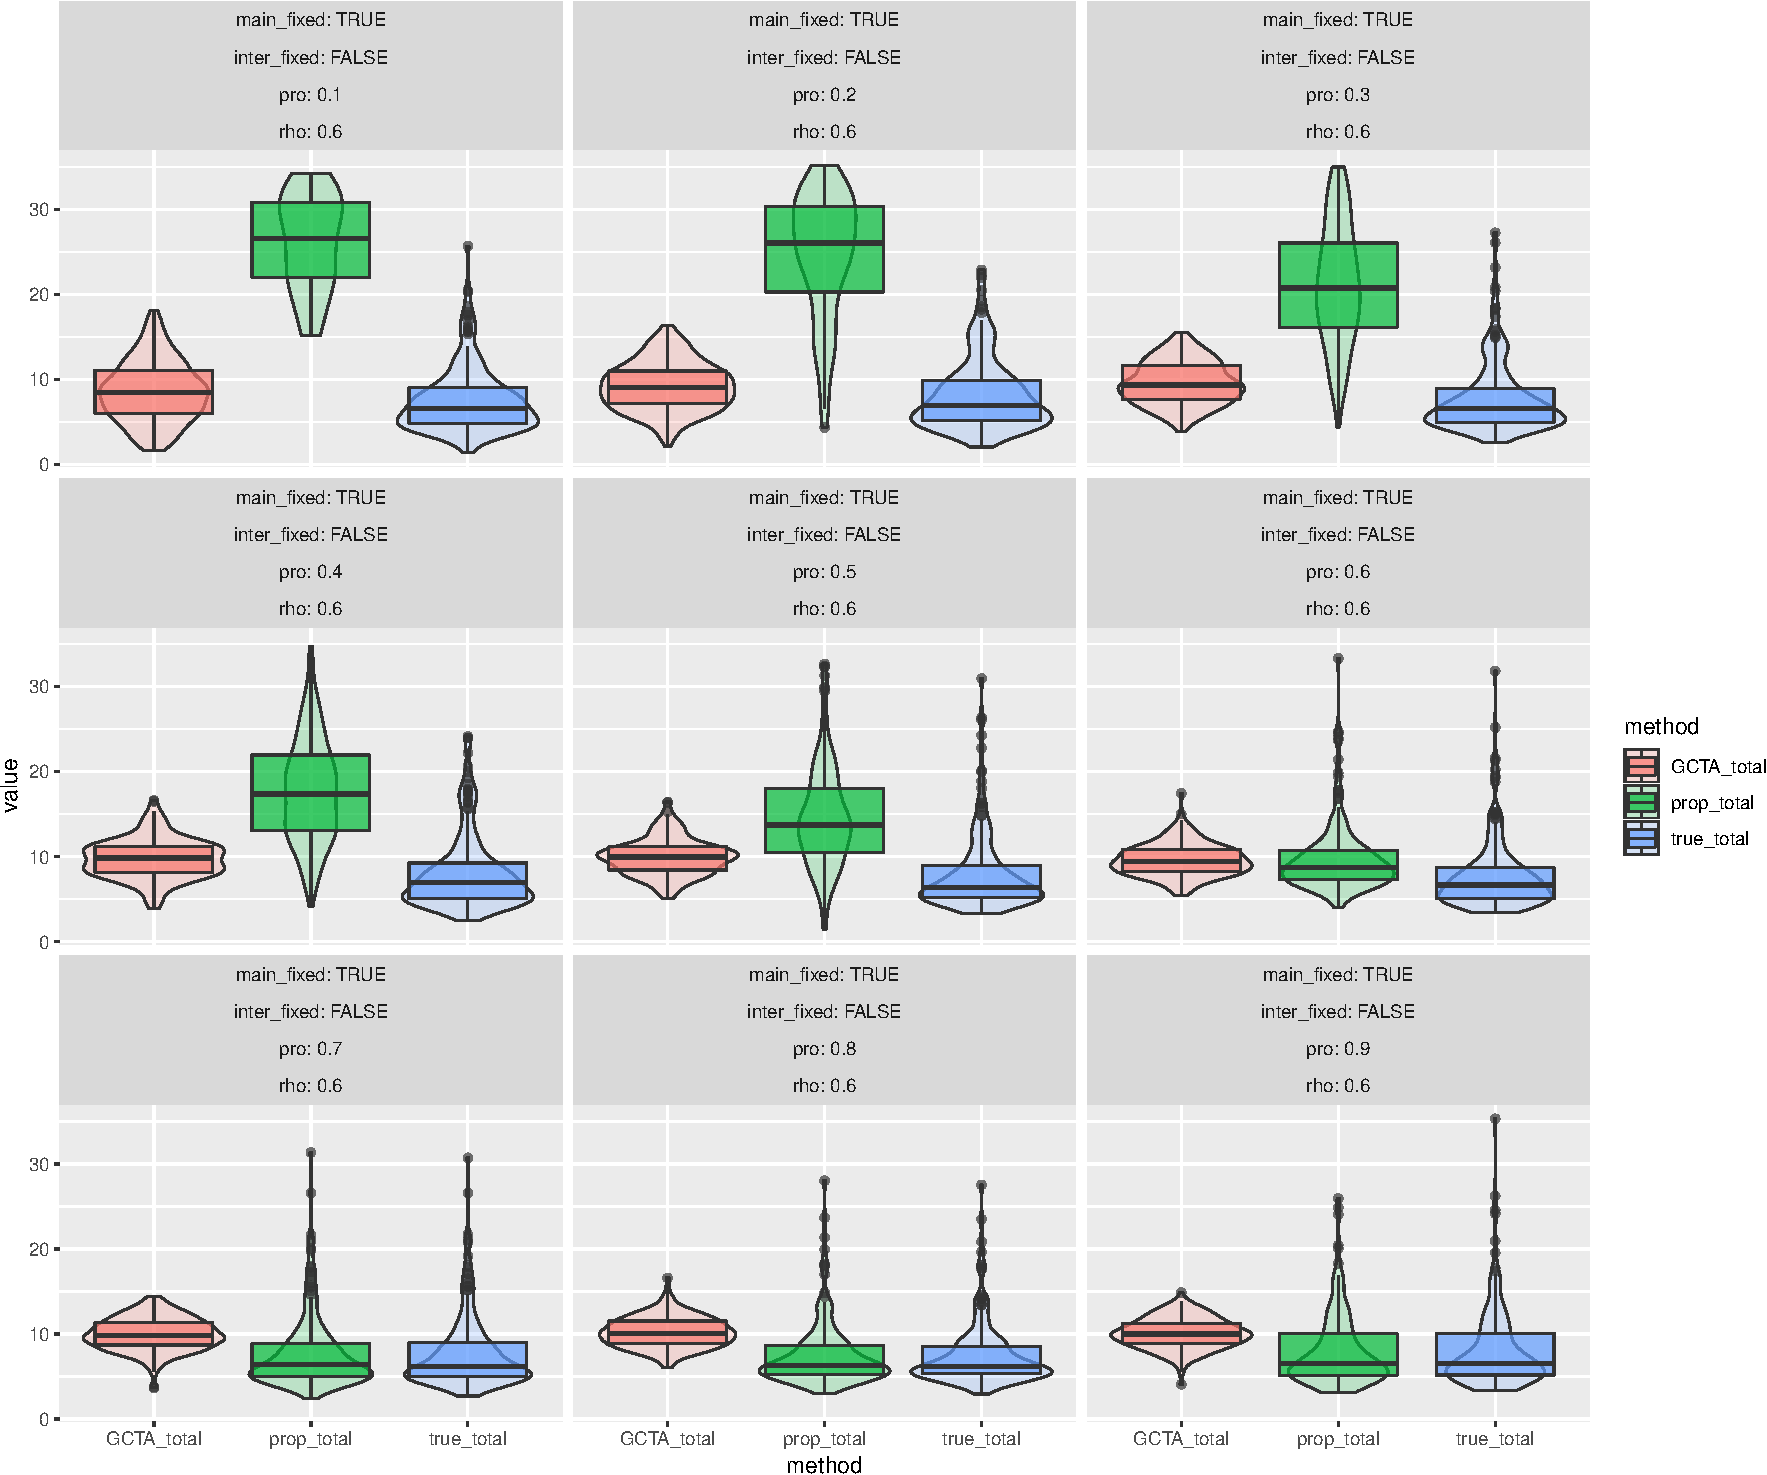
\includegraphics{Simulation_report_chi_resamle_files/figure-latex/fixed fixed-1.pdf}

\subsubsection{fixed main and random interactive
effect}\label{fixed-main-and-random-interactive-effect}

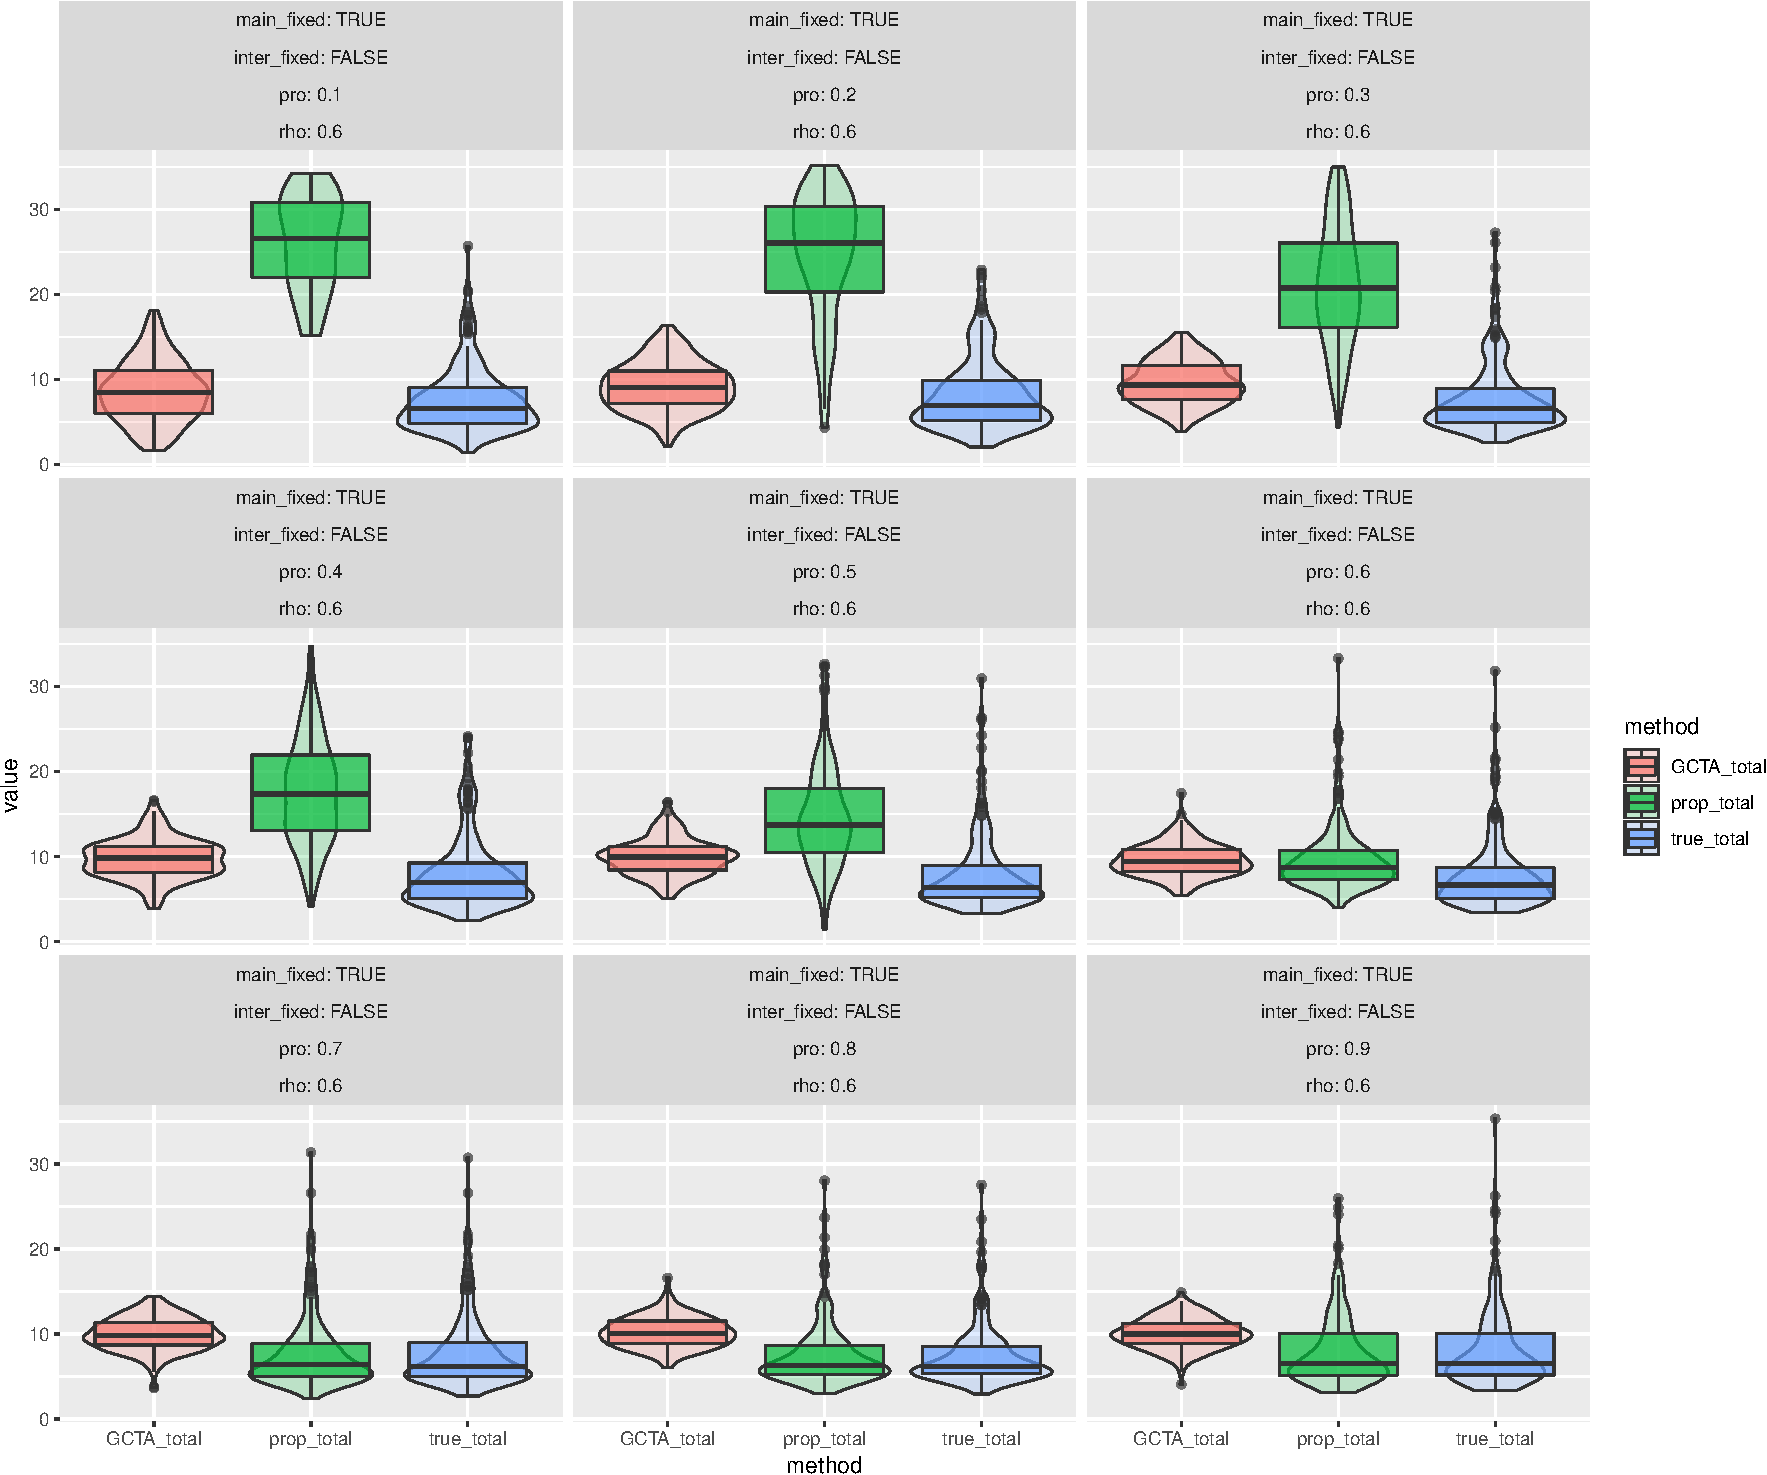
\includegraphics{Simulation_report_chi_resamle_files/figure-latex/fixed random-1.pdf}

\subsubsection{random main and random interactive
effect}\label{random-main-and-random-interactive-effect}

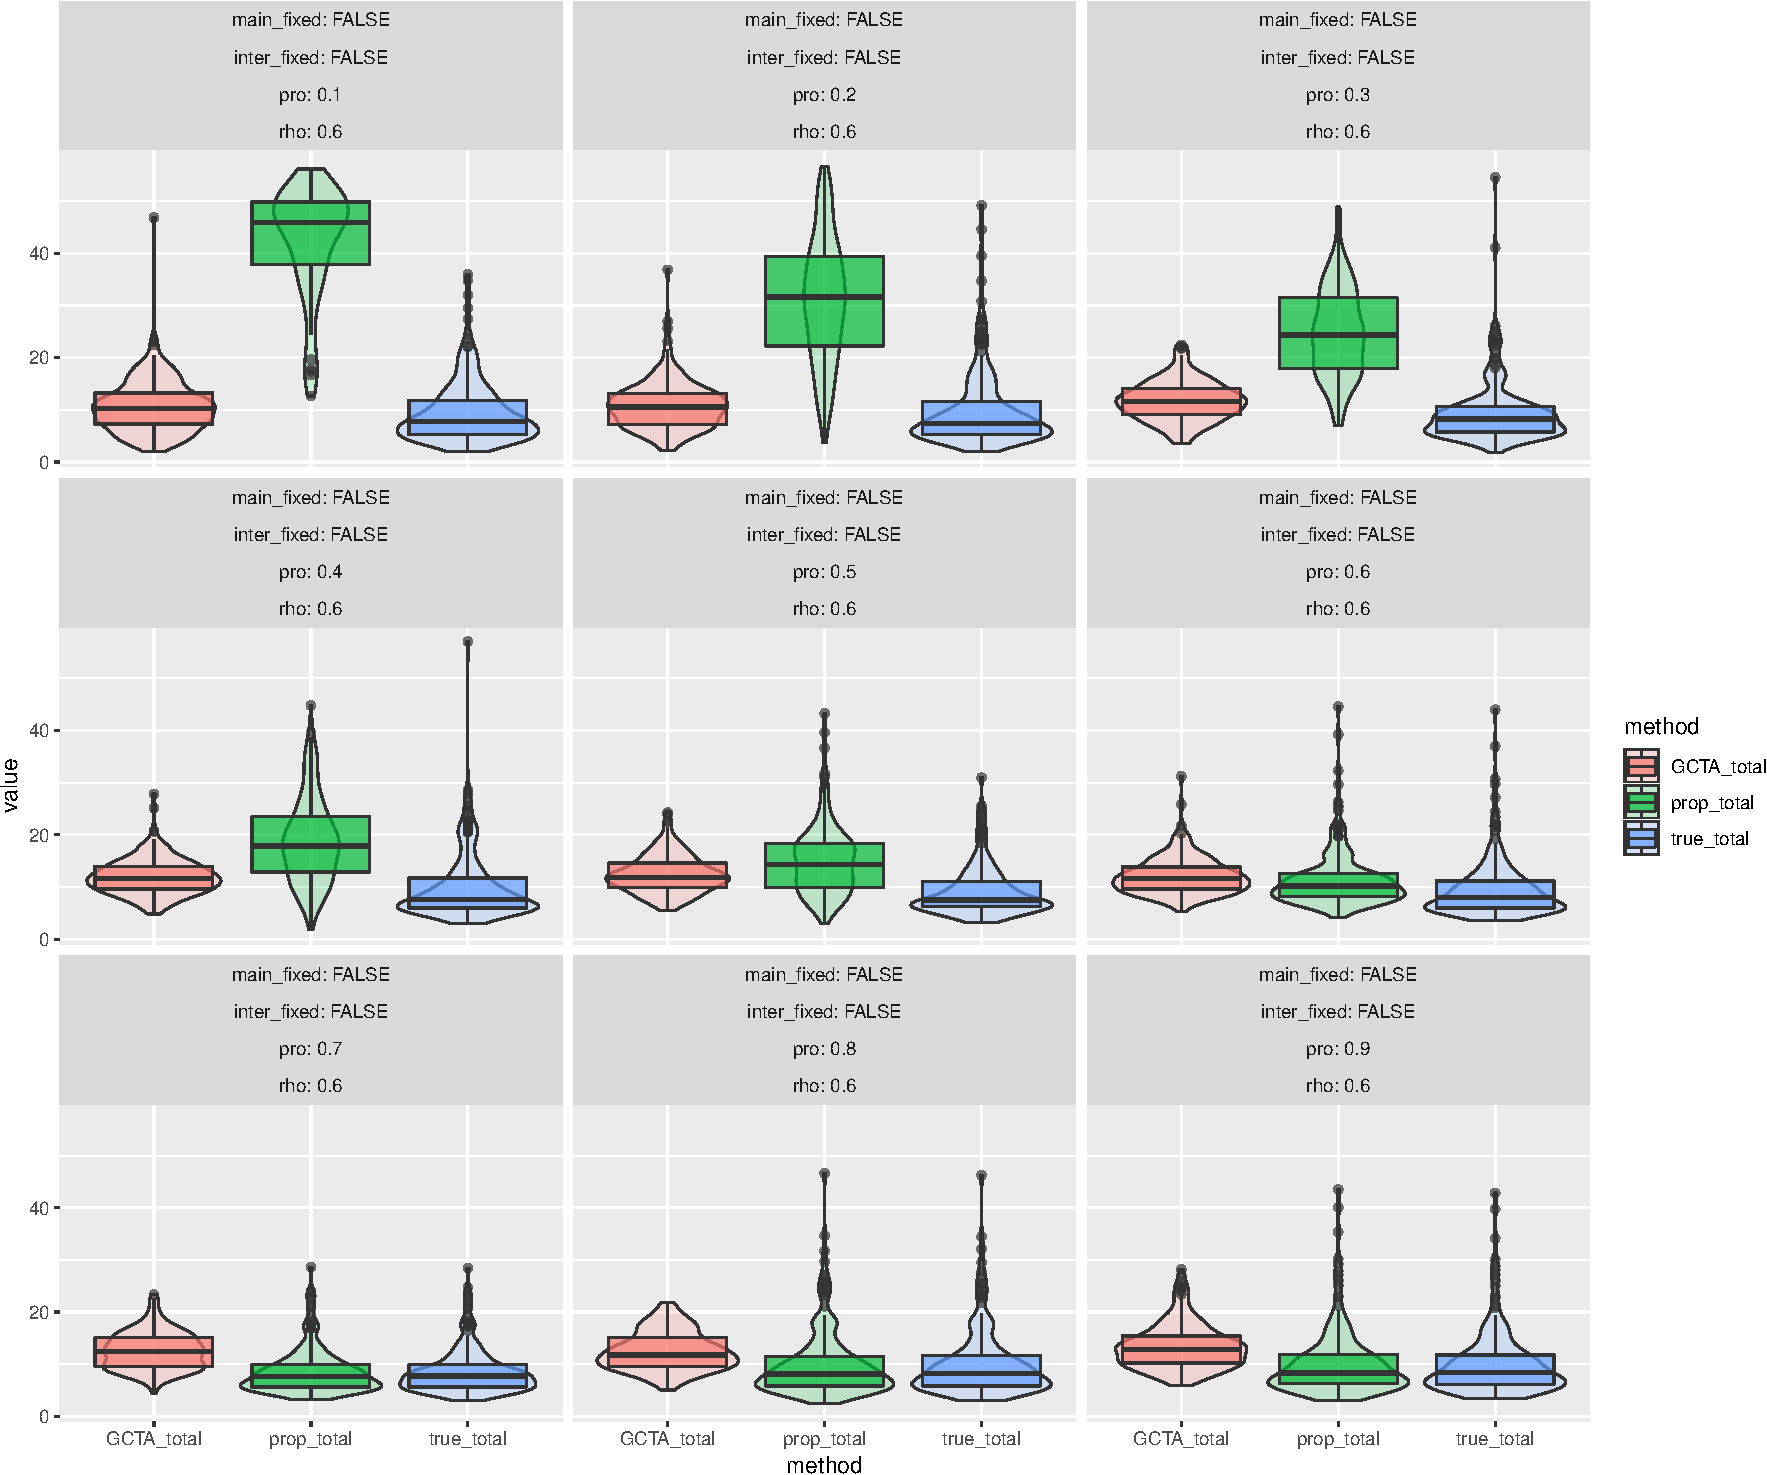
\includegraphics{Simulation_report_chi_resamle_files/figure-latex/random random-1.pdf}

\subsection{p = 6}\label{p-6}

\subsubsection{fixed main and fixed interactive effect with p =
6}\label{fixed-main-and-fixed-interactive-effect-with-p-6}

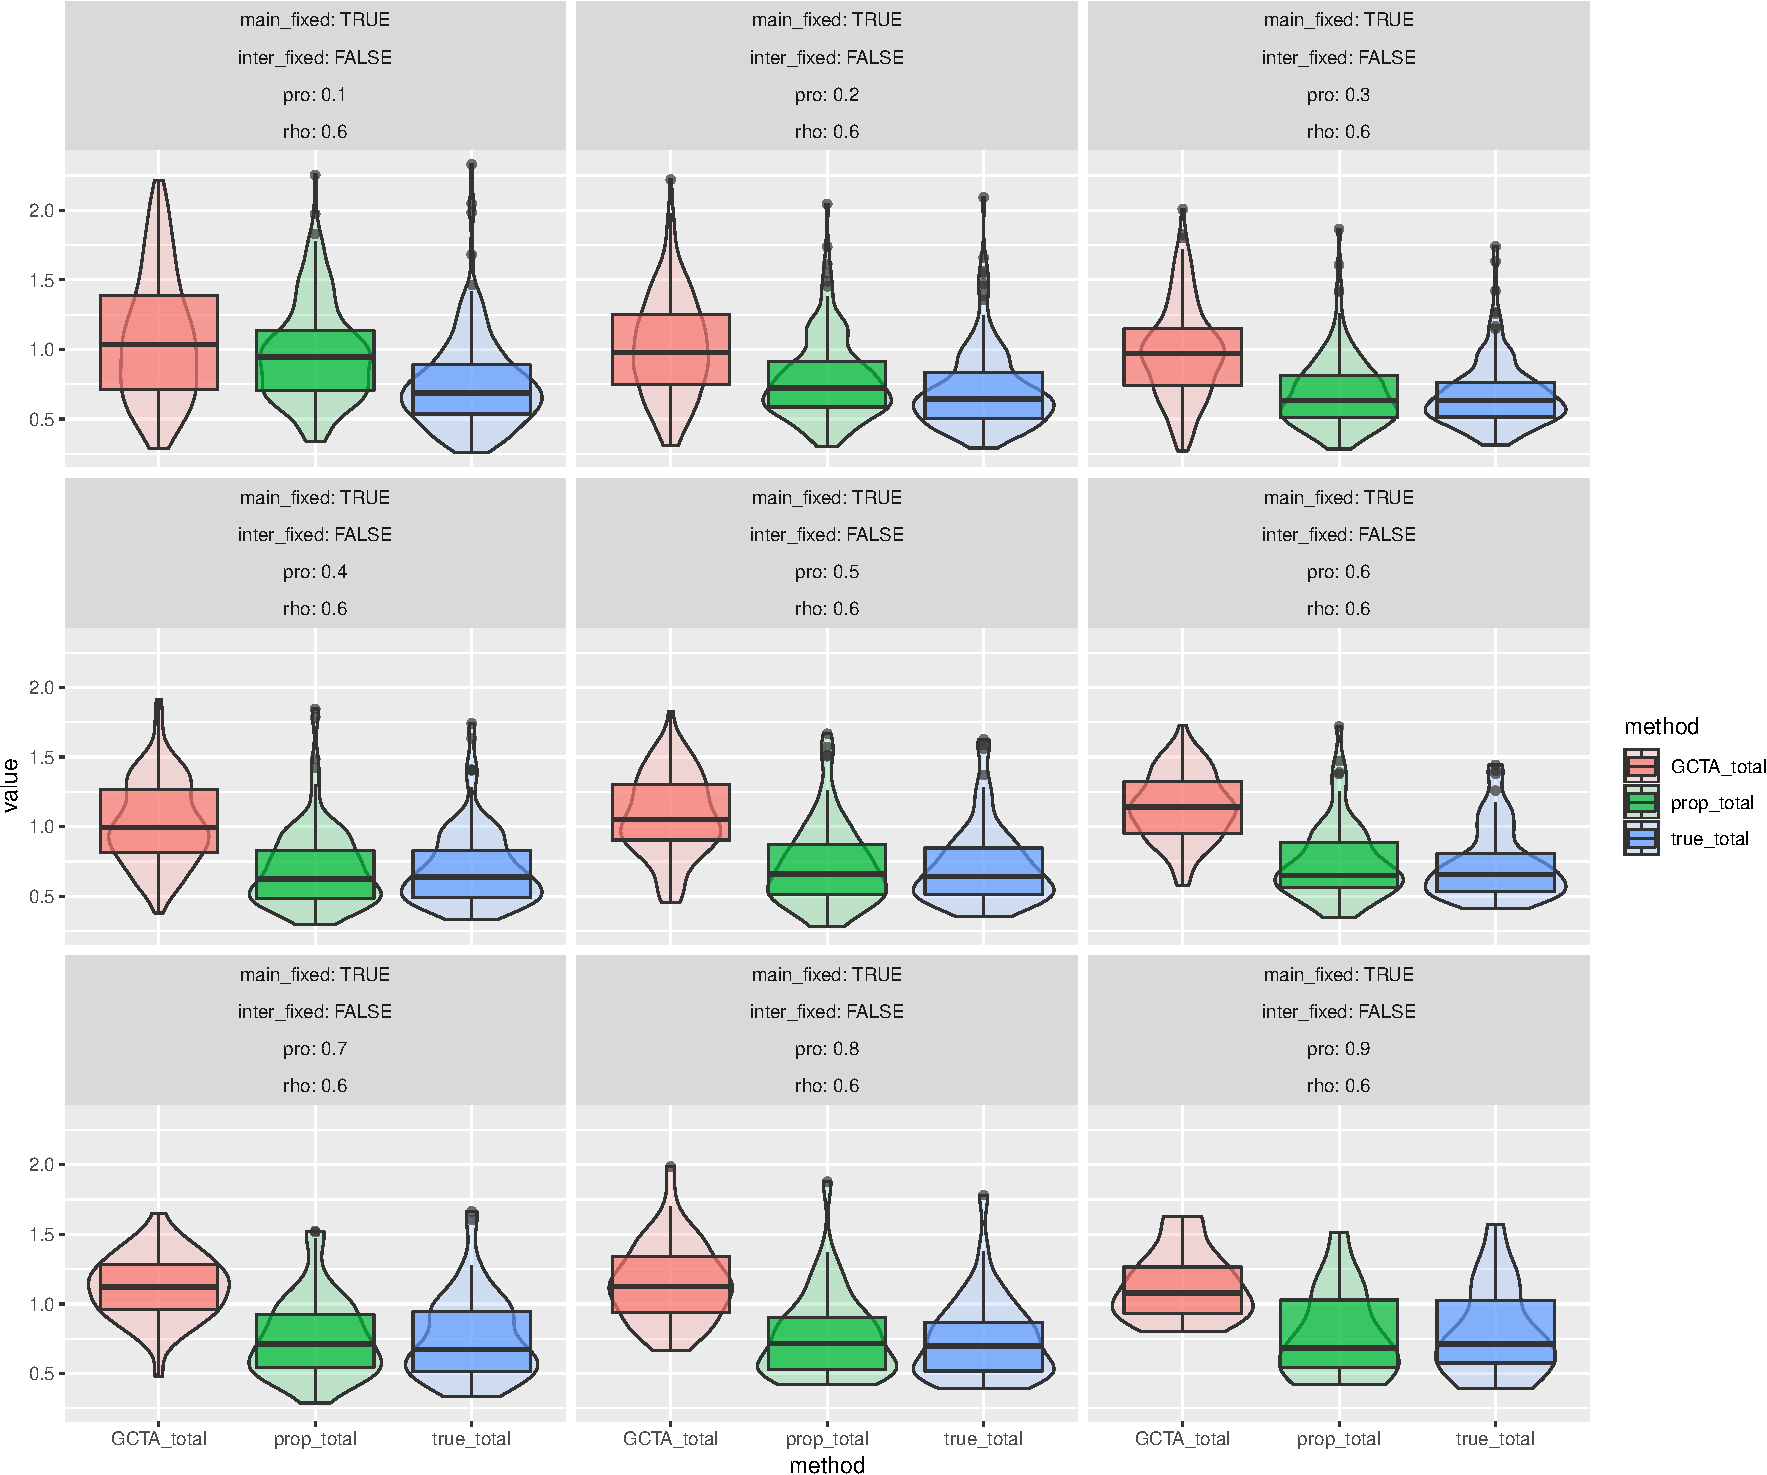
\includegraphics{Simulation_report_chi_resamle_files/figure-latex/fixed fixed p 6-1.pdf}

\subsubsection{fixed main and random interactive effect with p =
6}\label{fixed-main-and-random-interactive-effect-with-p-6}

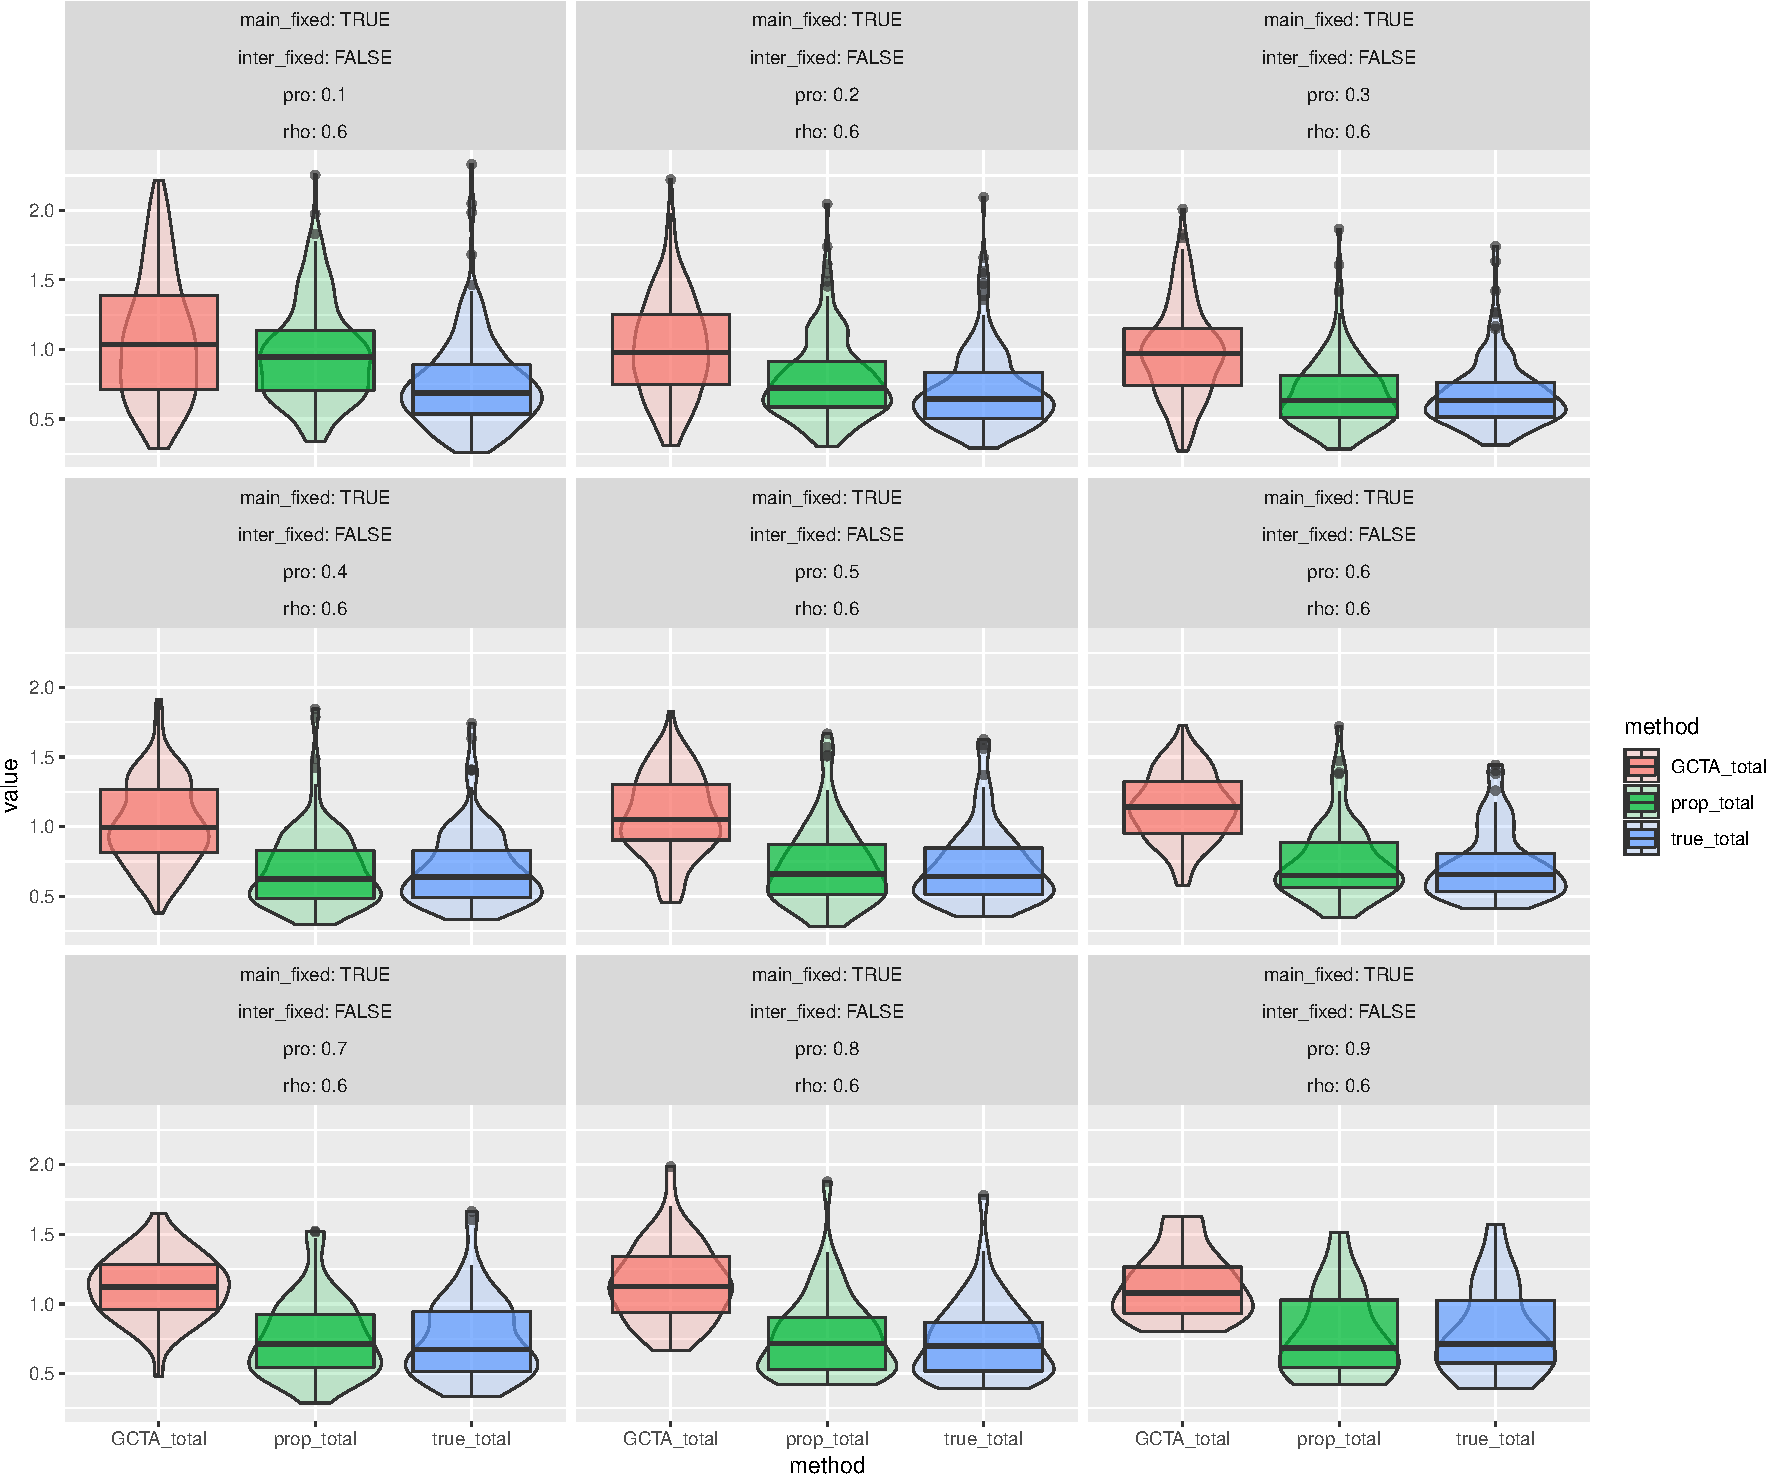
\includegraphics{Simulation_report_chi_resamle_files/figure-latex/fixed random p 6-1.pdf}

\subsubsection{random main and random interactive effect with p =
6}\label{random-main-and-random-interactive-effect-with-p-6}

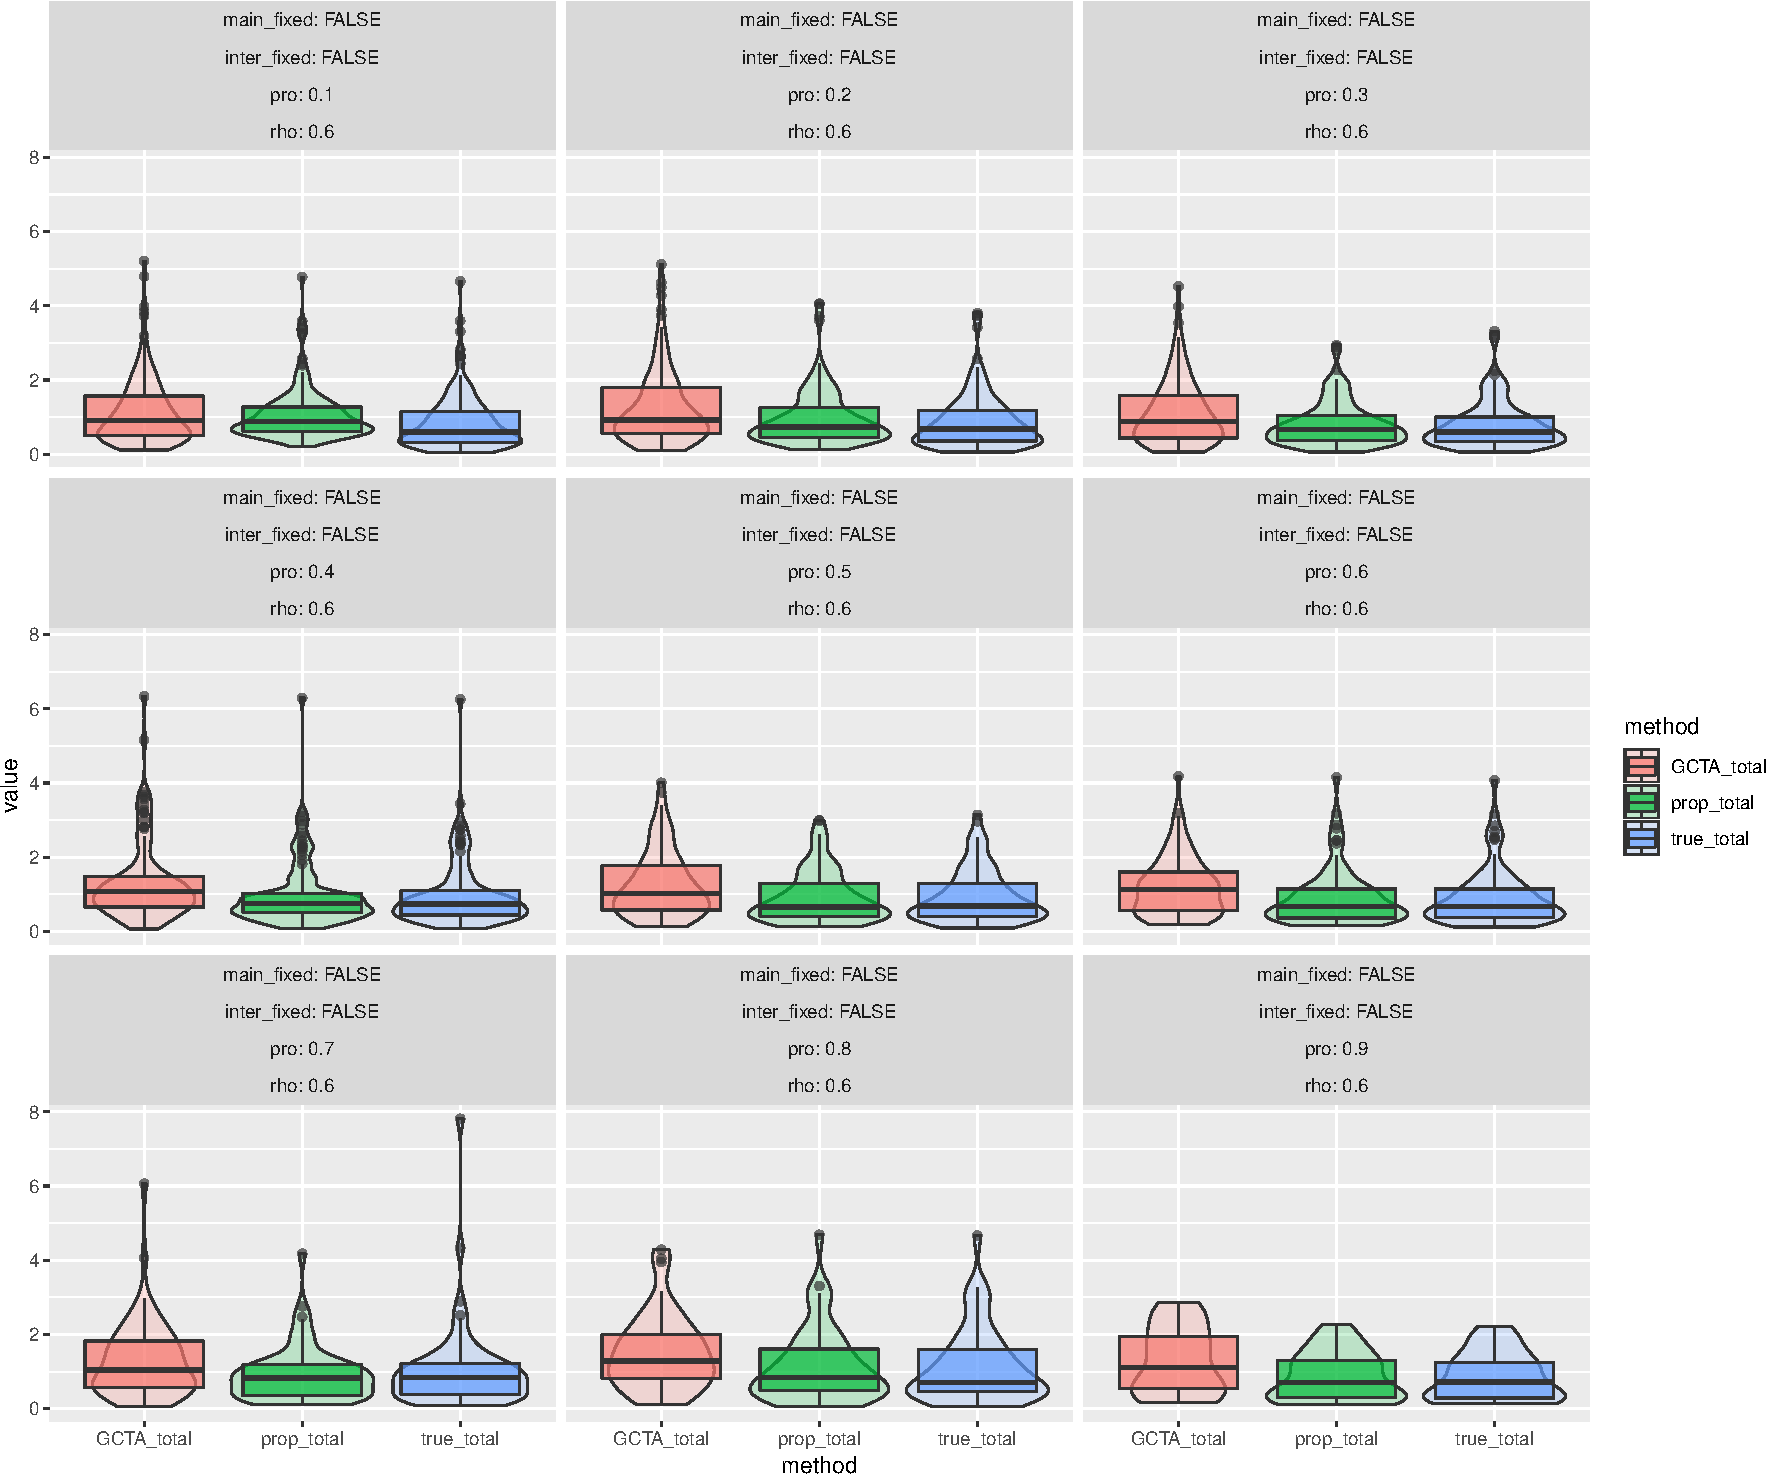
\includegraphics{Simulation_report_chi_resamle_files/figure-latex/random random p 6-1.pdf}

\subsection{only decorrelated main
effect}\label{only-decorrelated-main-effect}

\subsubsection{fixed main and fixed interactive
effect}\label{fixed-main-and-fixed-interactive-effect-1}

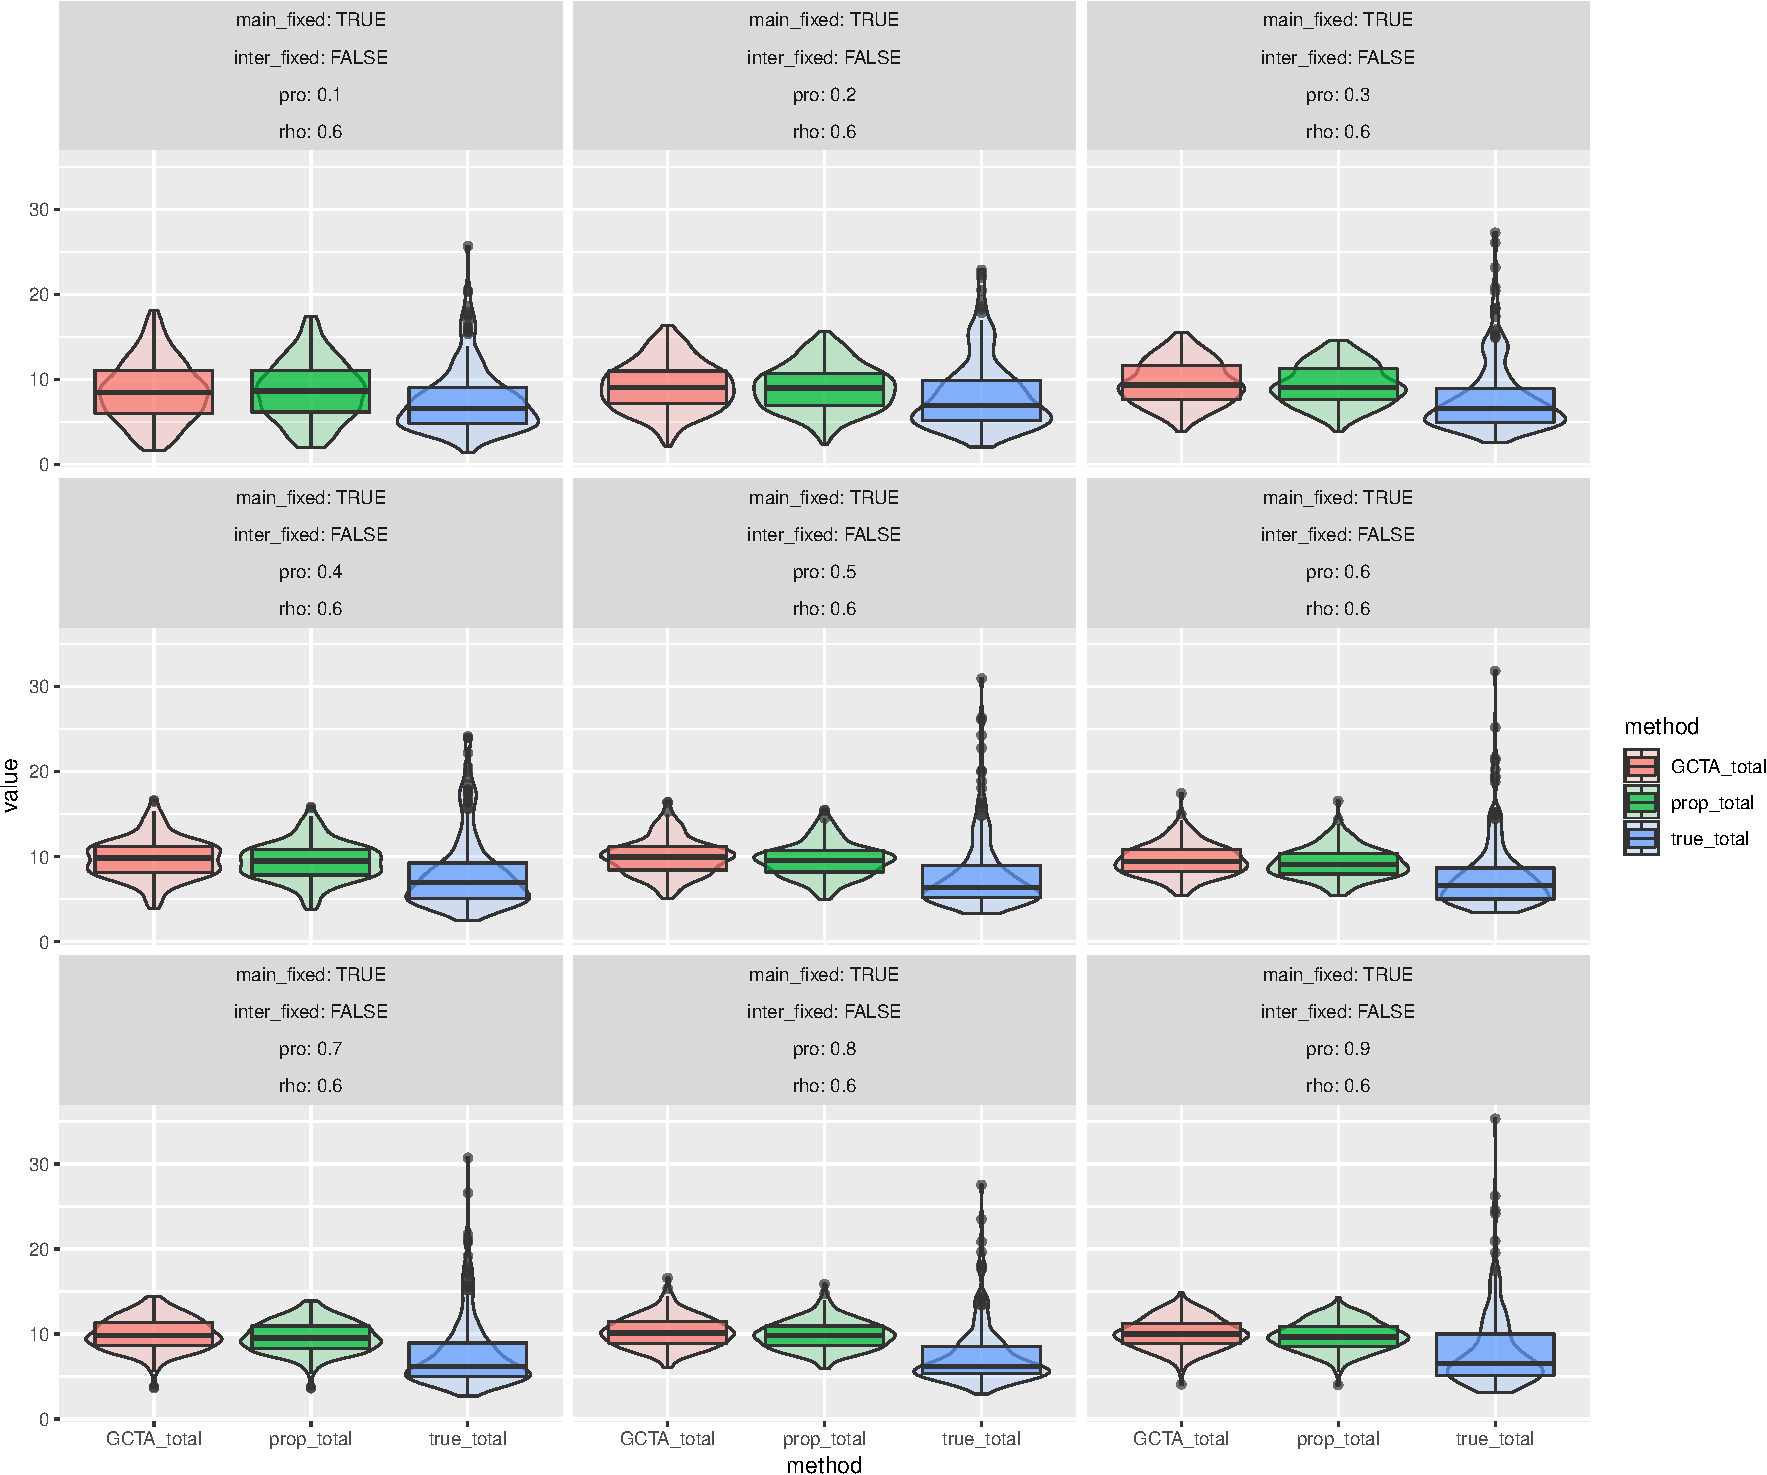
\includegraphics{Simulation_report_chi_resamle_files/figure-latex/fixed fixed decorr main-1.pdf}

\subsubsection{fixed main and random interactive
effect}\label{fixed-main-and-random-interactive-effect-1}

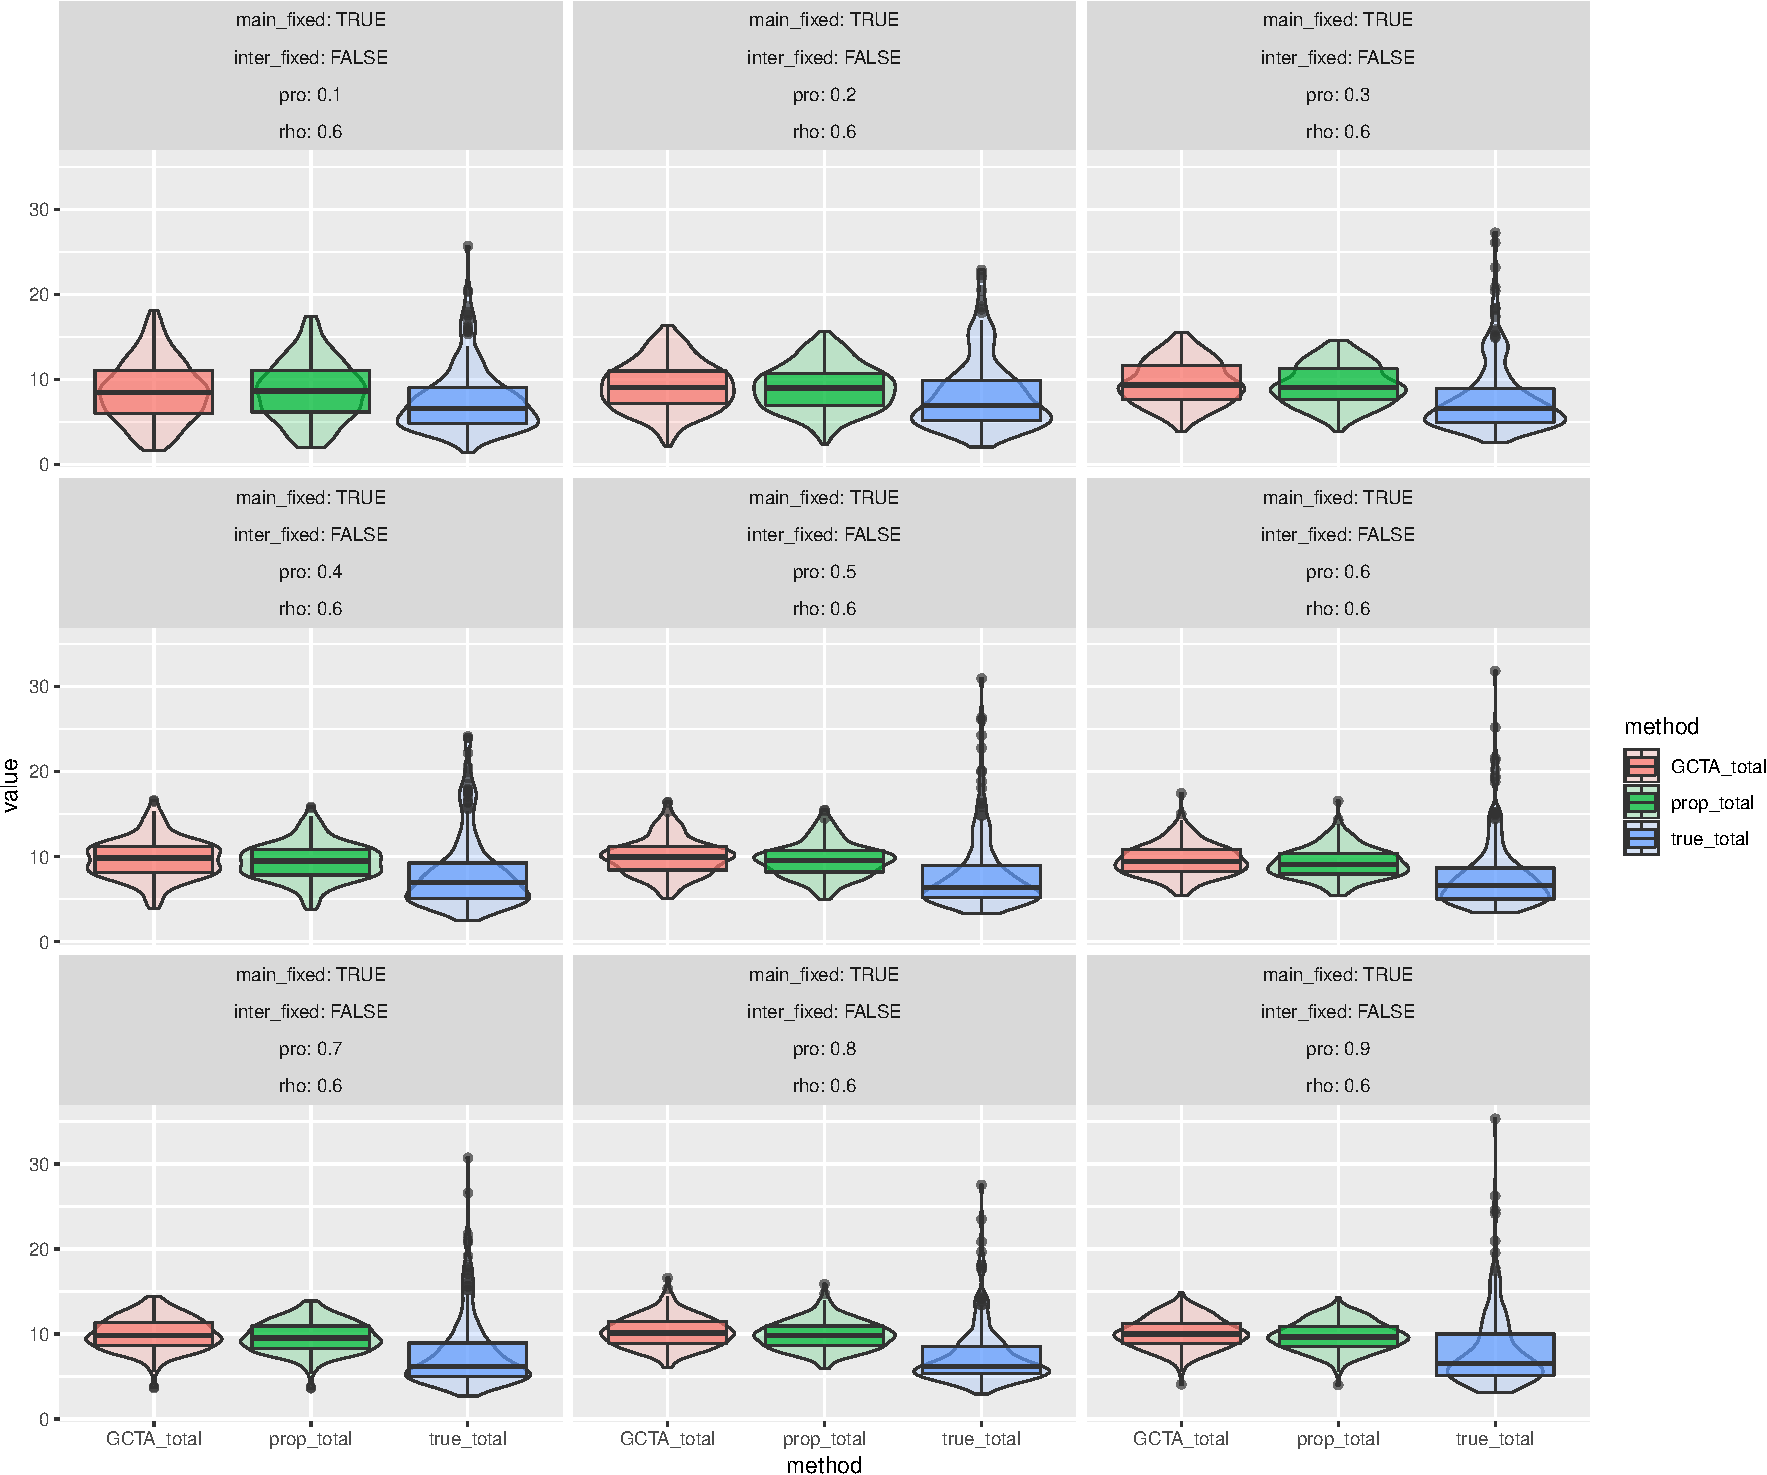
\includegraphics{Simulation_report_chi_resamle_files/figure-latex/fixed random decorr main-1.pdf}

\subsubsection{random main and random interactive
effect}\label{random-main-and-random-interactive-effect-1}

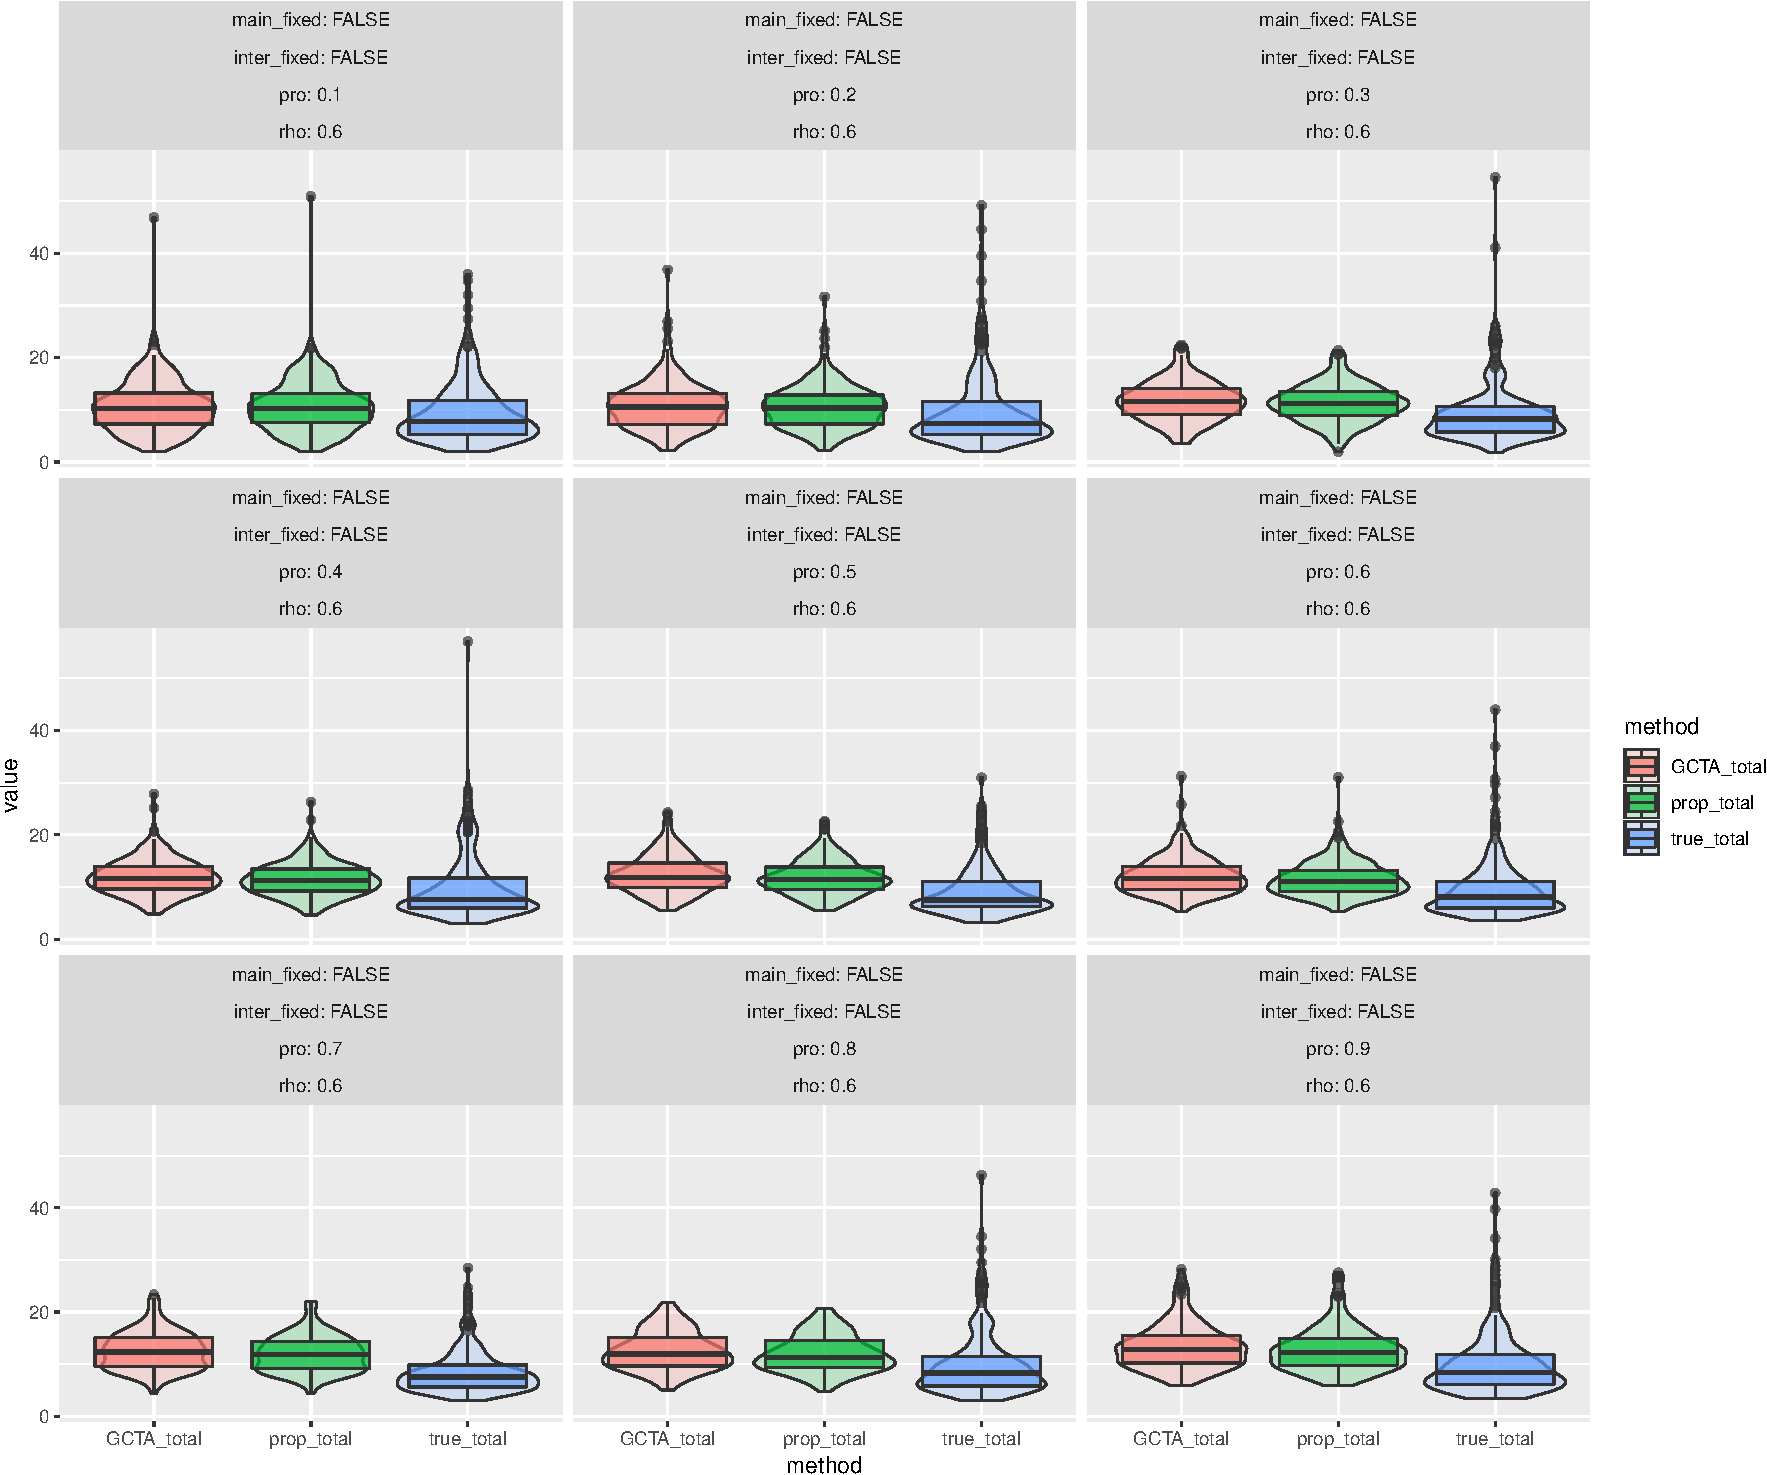
\includegraphics{Simulation_report_chi_resamle_files/figure-latex/random random decorr main-1.pdf}

\section{Conclusion}\label{conclusion}

\section{Further work}\label{further-work}


\end{document}
